\documentclass[../../FisicaTeorica.tex]{subfiles}


\begin{document}

\section{Scattering}

Discutiamo ora il caso di diffusione elastica da un bersaglio con la
finalit{\`a} di ottenere informazioni sulle forze a priori ignote esercitate
sulle particelle incidenti, stabilendo un legame tra potenziale incognito $V$ e i dati sperimentali che si esprimono in termini di sezione
d'urto.

Vediamo dunque l'esperimento di diffusione (scattering). Si consideri un
fascio di particelle identiche con momenti abbastanza ben focalizzati attorno
ad un valor medio $\vec{p}_0$ contro un bersaglio fisso con un certo numero di
centri di diffusione; il bersaglio {\`e} posto ad una distanza $D_0$ rispetto
al raggio d'azione delle forze, mentre i rivelatori sono posizionati a grande
distanza $D$ dal bersaglio (Figura \ref{fig:scattering1}).

\begin{figure}
    \centering
\tikzset{every picture/.style={line width=0.75pt}} %set default line width to 0.75pt        

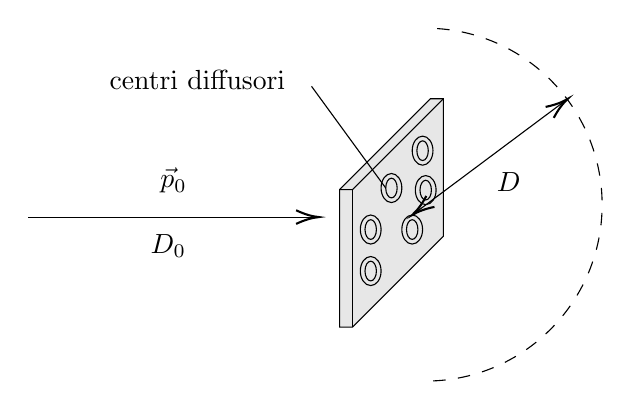
\begin{tikzpicture}[x=0.75pt,y=0.75pt,yscale=-1,xscale=1]
%uncomment if require: \path (0,213); %set diagram left start at 0, and has height of 213

%Straight Lines [id:da3904013711433083] 
\draw    (150,111) -- (288,111) ;
\draw [shift={(290,111)}, rotate = 180] [color={rgb, 255:red, 0; green, 0; blue, 0 }  ][line width=0.75]    (10.93,-3.29) .. controls (6.95,-1.4) and (3.31,-0.3) .. (0,0) .. controls (3.31,0.3) and (6.95,1.4) .. (10.93,3.29)   ;

%Shape: Cube [id:dp8271164620822671] 
\draw  [fill={rgb, 255:red, 231; green, 231; blue, 231 }  ,fill opacity=1 ] (300,97.75) -- (343.75,54) -- (350,54) -- (350,120.25) -- (306.25,164) -- (300,164) -- cycle ; \draw   (350,54) -- (306.25,97.75) -- (300,97.75) ; \draw   (306.25,97.75) -- (306.25,164) ;
%Shape: Donut [id:dp3395501450286591] 
\draw   (312.25,137) .. controls (312.25,134.38) and (313.48,132.25) .. (315,132.25) .. controls (316.52,132.25) and (317.75,134.38) .. (317.75,137) .. controls (317.75,139.62) and (316.52,141.75) .. (315,141.75) .. controls (313.48,141.75) and (312.25,139.62) .. (312.25,137)(310,137) .. controls (310,133.13) and (312.24,130) .. (315,130) .. controls (317.76,130) and (320,133.13) .. (320,137) .. controls (320,140.87) and (317.76,144) .. (315,144) .. controls (312.24,144) and (310,140.87) .. (310,137) ;
%Shape: Donut [id:dp30832634565439165] 
\draw   (312.25,117) .. controls (312.25,114.38) and (313.48,112.25) .. (315,112.25) .. controls (316.52,112.25) and (317.75,114.38) .. (317.75,117) .. controls (317.75,119.62) and (316.52,121.75) .. (315,121.75) .. controls (313.48,121.75) and (312.25,119.62) .. (312.25,117)(310,117) .. controls (310,113.13) and (312.24,110) .. (315,110) .. controls (317.76,110) and (320,113.13) .. (320,117) .. controls (320,120.87) and (317.76,124) .. (315,124) .. controls (312.24,124) and (310,120.87) .. (310,117) ;
%Shape: Donut [id:dp6521504490262637] 
\draw   (322.25,97) .. controls (322.25,94.38) and (323.48,92.25) .. (325,92.25) .. controls (326.52,92.25) and (327.75,94.38) .. (327.75,97) .. controls (327.75,99.62) and (326.52,101.75) .. (325,101.75) .. controls (323.48,101.75) and (322.25,99.62) .. (322.25,97)(320,97) .. controls (320,93.13) and (322.24,90) .. (325,90) .. controls (327.76,90) and (330,93.13) .. (330,97) .. controls (330,100.87) and (327.76,104) .. (325,104) .. controls (322.24,104) and (320,100.87) .. (320,97) ;
%Shape: Donut [id:dp4413746129647962] 
\draw   (332.25,117) .. controls (332.25,114.38) and (333.48,112.25) .. (335,112.25) .. controls (336.52,112.25) and (337.75,114.38) .. (337.75,117) .. controls (337.75,119.62) and (336.52,121.75) .. (335,121.75) .. controls (333.48,121.75) and (332.25,119.62) .. (332.25,117)(330,117) .. controls (330,113.13) and (332.24,110) .. (335,110) .. controls (337.76,110) and (340,113.13) .. (340,117) .. controls (340,120.87) and (337.76,124) .. (335,124) .. controls (332.24,124) and (330,120.87) .. (330,117) ;
%Shape: Donut [id:dp513426779404851] 
\draw   (337.25,79) .. controls (337.25,76.38) and (338.48,74.25) .. (340,74.25) .. controls (341.52,74.25) and (342.75,76.38) .. (342.75,79) .. controls (342.75,81.62) and (341.52,83.75) .. (340,83.75) .. controls (338.48,83.75) and (337.25,81.62) .. (337.25,79)(335,79) .. controls (335,75.13) and (337.24,72) .. (340,72) .. controls (342.76,72) and (345,75.13) .. (345,79) .. controls (345,82.87) and (342.76,86) .. (340,86) .. controls (337.24,86) and (335,82.87) .. (335,79) ;
%Shape: Donut [id:dp24956287073986094] 
\draw   (338.75,98) .. controls (338.75,95.38) and (339.98,93.25) .. (341.5,93.25) .. controls (343.02,93.25) and (344.25,95.38) .. (344.25,98) .. controls (344.25,100.62) and (343.02,102.75) .. (341.5,102.75) .. controls (339.98,102.75) and (338.75,100.62) .. (338.75,98)(336.5,98) .. controls (336.5,94.13) and (338.74,91) .. (341.5,91) .. controls (344.26,91) and (346.5,94.13) .. (346.5,98) .. controls (346.5,101.87) and (344.26,105) .. (341.5,105) .. controls (338.74,105) and (336.5,101.87) .. (336.5,98) ;
%Shape: Arc [id:dp43855429458278294] 
\draw  [draw opacity=0][dash pattern={on 4.5pt off 4.5pt}] (345.07,189.93) .. controls (390.36,188.05) and (426.5,150.75) .. (426.5,105) .. controls (426.5,58.55) and (389.24,20.8) .. (342.97,20.01) -- (341.5,105) -- cycle ; \draw  [dash pattern={on 4.5pt off 4.5pt}] (345.07,189.93) .. controls (390.36,188.05) and (426.5,150.75) .. (426.5,105) .. controls (426.5,58.55) and (389.24,20.8) .. (342.97,20.01) ;
%Straight Lines [id:da8415839157100764] 
\draw    (336.6,108.8) -- (408.4,55.2) ;
\draw [shift={(410,54)}, rotate = 503.25] [color={rgb, 255:red, 0; green, 0; blue, 0 }  ][line width=0.75]    (10.93,-3.29) .. controls (6.95,-1.4) and (3.31,-0.3) .. (0,0) .. controls (3.31,0.3) and (6.95,1.4) .. (10.93,3.29)   ;
\draw [shift={(335,110)}, rotate = 323.25] [color={rgb, 255:red, 0; green, 0; blue, 0 }  ][line width=0.75]    (10.93,-3.29) .. controls (6.95,-1.4) and (3.31,-0.3) .. (0,0) .. controls (3.31,0.3) and (6.95,1.4) .. (10.93,3.29)   ;
%Straight Lines [id:da8639267937604509] 
\draw    (286.5,48) -- (322.25,97) ;



% Text Node
\draw (220,93.5) node   {$\vec{p}_{0}$};
% Text Node
\draw (217.5,125) node   {$D_{0}$};
% Text Node
\draw (381.5,94) node   {$D$};
% Text Node
\draw (231.5,45) node  [align=left] {centri diffusori};

\end{tikzpicture}
    \caption{Schema esemplificativo dello scattering.}
    \label{fig:scattering1}
\end{figure}

Sia $a$ l'ampiezza del centro
diffusore.

Si assumono le seguenti ipotesi:
\begin{enumerate}
  \item si considerano solo urti elastici;
  
  \item si suppone che la distanza tra i centri diffusori sia maggiore di $a$
  e che il bersaglio sia abbastanza sottile in modo che la particella
  interagisca con {\tmem{un solo}} centro diffusore.
\end{enumerate}
Ad una grande distanza $D \gg a$ e a diversi angoli sono disposti i rivelatori
che conteggiano il numero di particelle diffuse dal bersaglio nell'unit{\`a}
di tempo sotto l'angolo solido $d \Omega (\theta, \varphi)$ nella direzione
$(\theta, \varphi)$ in un sistema di riferimento che ha origine nel centro
delle forze con coordinate polari (Figura \ref{fig:scattering2}).

\begin{figure}
    \centering


\tikzset{every picture/.style={line width=0.75pt}} %set default line width to 0.75pt        

\begin{tikzpicture}[x=0.75pt,y=0.75pt,yscale=-1,xscale=1]
%uncomment if require: \path (0,213); %set diagram left start at 0, and has height of 213

%Straight Lines [id:da486245224033673] 
\draw    (150,111) -- (288,111) ;
\draw [shift={(290,111)}, rotate = 180] [color={rgb, 255:red, 0; green, 0; blue, 0 }  ][line width=0.75]    (10.93,-3.29) .. controls (6.95,-1.4) and (3.31,-0.3) .. (0,0) .. controls (3.31,0.3) and (6.95,1.4) .. (10.93,3.29)   ;

%Shape: Donut [id:dp4674326715344803] 
\draw   (302.25,110) .. controls (302.25,105.72) and (303.48,102.25) .. (305,102.25) .. controls (306.52,102.25) and (307.75,105.72) .. (307.75,110) .. controls (307.75,114.28) and (306.52,117.75) .. (305,117.75) .. controls (303.48,117.75) and (302.25,114.28) .. (302.25,110)(300,110) .. controls (300,104.48) and (302.24,100) .. (305,100) .. controls (307.76,100) and (310,104.48) .. (310,110) .. controls (310,115.52) and (307.76,120) .. (305,120) .. controls (302.24,120) and (300,115.52) .. (300,110) ;
%Shape: Arc [id:dp9798656347840484] 
\draw  [draw opacity=0][dash pattern={on 4.5pt off 4.5pt}] (311.32,194.93) .. controls (356.61,193.05) and (392.75,155.75) .. (392.75,110) .. controls (392.75,63.55) and (355.49,25.8) .. (309.22,25.01) -- (307.75,110) -- cycle ; \draw  [dash pattern={on 4.5pt off 4.5pt}] (311.32,194.93) .. controls (356.61,193.05) and (392.75,155.75) .. (392.75,110) .. controls (392.75,63.55) and (355.49,25.8) .. (309.22,25.01) ;
%Straight Lines [id:da23525789815849873] 
\draw    (305,110) -- (370,50) ;
\draw [shift={(370,50)}, rotate = 362.29] [color={rgb, 255:red, 0; green, 0; blue, 0 }  ][line width=0.75]    (-5.59,0) -- (5.59,0)(0,5.59) -- (0,-5.59)   ;

%Straight Lines [id:da3930829180952482] 
\draw  [dash pattern={on 0.84pt off 2.51pt}]  (307.75,110) -- (434.5,110) ;
\draw [shift={(436.5,110)}, rotate = 180] [color={rgb, 255:red, 0; green, 0; blue, 0 }  ][line width=0.75]    (10.93,-3.29) .. controls (6.95,-1.4) and (3.31,-0.3) .. (0,0) .. controls (3.31,0.3) and (6.95,1.4) .. (10.93,3.29)   ;

%Curve Lines [id:da328048332083702] 
\draw    (331.76,88.77) .. controls (339.45,96.25) and (339.81,100.69) .. (340,110) ;

\draw [shift={(330.2,87.3)}, rotate = 42.4] [fill={rgb, 255:red, 0; green, 0; blue, 0 }  ][line width=0.75]  [draw opacity=0] (8.93,-4.29) -- (0,0) -- (8.93,4.29) -- cycle    ;
%Curve Lines [id:da256666836269986] 
\draw    (373.67,115.78) .. controls (372.12,134.04) and (360.21,127.44) .. (360.6,109.3) .. controls (361,90.5) and (373.3,87.25) .. (373.6,102.8) ;

\draw [shift={(373.8,113.7)}, rotate = 92.2] [fill={rgb, 255:red, 0; green, 0; blue, 0 }  ][line width=0.75]  [draw opacity=0] (8.93,-4.29) -- (0,0) -- (8.93,4.29) -- cycle    ;

% Text Node
\draw (220,93.5) node   {$\vec{p}_{0}$};
% Text Node
\draw (217.5,125) node   {$D_{0}$};
% Text Node
\draw (327,100) node   {$\theta $};
% Text Node
\draw (370,79) node   {$\varphi $};
% Text Node
\draw (431.5,92.5) node   {$z$};
% Text Node
\draw (407,40.5) node  [align=left] {rivelatore};


\end{tikzpicture}
    \caption{Schema delle coordinate angolari per lo scattering.}
    \label{fig:scattering2}
\end{figure}

Sia $\Phi_i$ il \tmtextit{flusso di particelle incidenti} (pedice $i$)
nell'unit{\`a} di tempo per unit{\`a} d'area. Denotiamo con $\vec{j}_i$ la
corrente corrispondente e con $\Phi_i = | \vec{j}_i |$. Si ha infatti
\[ \Phi_i = \frac{d^{} N_i}{d^{} S d^{} t} = \frac{d^{} N_i}{\underbrace{d^{}
   S \hspace{0.17em} d^{} z}_{dV}}  \frac{d^{} z}{d^{} t} = n_i v_i = j_i = |
   \vec{j}_i | \]
dove $dN_i$ {\`e} il numero di particelle incidenti, $dS$ l'unit{\`a} d'area
trasversa a $\vec{p}_0$ e $n_i$ {\`e} la densit{\`a} di particelle incidenti.

Sia $\Phi_d (\theta, \varphi)$ il \tmtextit{flusso di particelle diffuse}
nell'unit{\`a} di tempo e nell'unit{\`a} di angolo solido nella direzione
$(\theta, \varphi)$. Denotiamo con $\vec{j}_d$ la corrente associata al flusso
tale che
\[ \Phi_d (\theta, \varphi) = r^2  | \vec{j}_d \cdot \hat{r} | \qquad
   \text{con} \quad \hat{r} = \frac{\vec{x}}{| \vec{x} |} \]
infatti si ha
\[ \Phi_d (\theta, \varphi) = \frac{d N (\theta, \varphi)}{d t \hspace{0.17em}
   d \Omega} = \frac{d N (\theta, \varphi)}{d \Omega \hspace{0.17em} r^2 
   \hspace{0.17em} d r} \cdot r^2  \frac{d r}{d t} = r^2  | \vec{j}_d \cdot
   \hat{r} | \]
La sezione d'urto {\`e} il rapporto tra i flussi diffuso e incidente. La
quantit{\`a}
\begin{equation}
\label{sezurtodiff} \sigma (\theta, \varphi) \equiv \frac{\Phi_d (\theta,
   \varphi)}{\Phi_i} = \frac{r^2  | \vec{j}_d \cdot \hat{r} |}{| \vec{j}_i |}
\end{equation}
{\`e} detta {\tmem{sezione d'urto differenziale}}, ed ha le dimensioni di
un'area. Si noti che  il rapporto \eqref{sezurtodiff} {\`e} indipendente dal numero $N$ di
particelle incidenti che ho mandato sul bersaglio, e le stesse definizioni e
formule per i flussi e sezione d'urto valgono anche nel caso delle correnti di
probabilit{\`a} per particella singola. Si ha infatti

\begin{align}
  \sigma (\theta, \varphi) & = \frac{\text{N. di partic. diffuse per unit{\`a}
  di tempo e angolo solido attorno a } (\theta, \varphi)}{\text{N. di partic.
  incidenti per unit{\`a} di tempo e di superficie}} \notag \\
  & = \frac{\text{Probabilit{\`a} di diffusione per angolo solido attorno a }
  (\theta, \varphi)}{\text{Probabilit{\`a} di incidenza per unit{\`a} di
  superficie}} \notag\\
  & = \frac{| \vec{j}_d \cdot \hat{r} | r^2}{| \vec{j}_i |} \label{sezurtodiff2}
\end{align}

dove in quest'ultima formula $\vec{j}$ assume appunto il significato di
corrente di probabilit{\`a}.

\subsection{Soluzioni stazionarie}

Supponiamo ora (e lo vedremo nel dettaglio in seguito) che una soluzione
dell'equazione di Schr{\"o}dinger stazionaria, fissato il momento incidente
$\vec{p}$, a grande distanza dal bersaglio abbia la forma asintotica
\begin{equation}
\label{formaasintotica}
\psi_{\text{as}} (\vec{x}, t) = e^{- \frac{i}{\hbar} \mathcal{E}t} (\psi_i
   + \psi_d) = e^{- \frac{i}{\hbar} \mathcal{E}t}  \left[
   \underbrace{e^{\frac{i}{\hbar}  \vec{p} \cdot \vec{x}}}_{= \psi_i} +
   \underbrace{f_{\vec{p}} (\theta, \varphi) \frac{e^{\frac{i}{\hbar}
   pr}}{r}}_{= \psi_d} \right]
\end{equation}
dove $p = | \vec{p} |$. La $\psi_i$ rappresenta la funzione d'onda della
particella prima dell'urto, mentre la $\psi_d$ {\`e} la funzione d'onda dopo
l'urto, modulata da una funzione $f$ che dipende dall'angolo di diffusione.
Siccome a grande distanza dal bersaglio la particella {\`e} libera sappiamo
perfettamente quanto vale l'energia $\mathcal{E}= p^2 / 2 m$. Lo spin
verr{\`a} trascurato nella discussione.

Consideriamo ora il caso di particella singola, dunque consideriamo le
correnti di probabilit{\`a}. Conoscendo la forma dell'onda di probabilit{\`a}
conosciamo anche la forma delle correnti di probabilit{\`a} direttamente dalla
loro definizione:
\begin{eqnarray*}
  \vec{j}_i & \equiv & \frac{\hbar}{2 m}  (\psi^{\ast}_i  \vec{\nabla} \psi_i
  - \vec{\nabla} \psi_i^{\ast} \psi_i)\\
  & = & \frac{\hbar}{2 m} 2 \text{Im} \{\psi_i^{\ast}  \vec{\nabla} \psi_i
  \}\\
  & = & \frac{\hbar}{m}  \text{Im} \{e^{- i \frac{\vec{p} \cdot
  \vec{x}}{\hbar}}  \vec{\nabla} e^{i \frac{\vec{p} \cdot \vec{x}}{\hbar}}
  \}\\
  & = & \frac{\hbar}{m}  \text{Im} \{e^{- i \frac{\vec{p} \cdot
  \vec{x}}{\hbar}}  \frac{\vec{p}}{\hbar} e^{i \frac{\vec{p} \cdot
  \vec{x}}{\hbar}} \}\\
  & = & \frac{\hbar}{m} \cdot \frac{\vec{p}}{\hbar} = \frac{\vec{p}}{m} =
  \vec{v}
\end{eqnarray*}
cio{\`e} si ottiene la velocit{\`a} della particella. Per $\vec{j}_d$ si ha
analogamente

\begin{align}
  | \vec{j}_d \cdot \hat{r} | & = \frac{\hbar}{m} \text{Im} [\psi_d^{\ast}
  \hspace{0.17em} \overbrace{\hat{r} \cdot \vec{\nabla}}^{\partial / \partial
  r} \psi_d] \notag \\
  & = \frac{\hbar}{m} \hspace{0.17em} \mathrm{Im} \left[ \psi_d^{\ast} 
  \frac{\partial}{\partial r} \psi_d \right] \notag \\
  & = \frac{\hbar}{m} \hspace{0.17em} \mathrm{Im} \left[ \left( f_{\vec{p}}
  (\theta, \varphi) \frac{e^{i \frac{pr}{\hbar}}}{r} \right)^{\ast} 
  \frac{\partial}{\partial r}  \left( f_{\vec{p}} (\theta, \varphi) \frac{e^{i
  \frac{pr}{\hbar}}}{r} \right) \right] \notag \\
  & = \frac{\hbar}{m} \hspace{0.17em} \mathrm{Im} \left[ f_{\vec{p}}^{\ast}
  (\theta, \varphi) f_{\vec{p}} (\theta, \varphi) \frac{e^{- i
  \frac{pr}{\hbar}}}{r}^{}  \frac{\partial}{\partial r}  \left( \frac{e^{i
  \frac{pr}{\hbar}}}{r} \right) \right] \notag \\
  & = \frac{\hbar}{m} \hspace{0.17em} \mathrm{Im} \left[ | f_{\vec{p}}
  (\theta, \varphi) |^2 \left( i \frac{p}{\hbar}  \frac{1}{r^2} -
  \frac{1}{r^3} \right) \right] \notag \\
  & = \frac{\hbar}{m}  | f_{\vec{p}} (\theta, \varphi) |^2  \frac{p}{\hbar} 
  \frac{1}{r^2} = v \frac{| f_{\vec{p}} (\theta, \varphi) |^2}{r^2} \notag
\end{align}

da cui si ottiene la sezione d'urto differenziale dalla definizione
{\eqref{sezurtodiff2}}:
\begin{equation}
  \label{sezurto1} \sigma (\theta, \varphi) = \frac{| \vec{j}_d \cdot \hat{r}
  | r^2}{| \vec{j}_i |} = \frac{v \frac{| f_{\vec{p}} (\theta, \varphi)
  |^2}{r^2} r^2}{v} = | f_{\vec{p}} (\theta, \varphi) |^2
\end{equation}


\subsection{Pacchetto d'onda incidente}

La trattazione precedente tuttavia non riproduce un processo fisico, dato che tale 
processo non {\`e} stazionario.
La situazione sperimentale {\`e}
costituita da particelle incidenti che sono libere molto prima che avvenga
l'urto ($t \to - \infty$), in cui siamo a grande distanza dal bersaglio, e
nuovamente libere molto dopo che avvenga l'urto ($t \to + \infty$), diffuse a
grande distanza. Tale funzione non {\`e} stazionaria. Notiamo inoltre che la
funzione d'onda \eqref{formaasintotica} che abbiamo costruito non {\`e} nemmeno in
$L^2$ (non rappresenta dunque uno stato fisico).

Per riprodurre la situazione fisica dobbiamo quindi considerare dei
\tmtextit{pacchetti d'onda} con le caratteristiche richieste: saranno
perci{\`o} formati con soluzioni stazionarie e riprodurranno comunque la
{\eqref{sezurto1}}, anche se in pi{\`u} apparir{\`a} una relazione tra $f$ e
il potenziale $V$ di interazione. La trattazione precedente, dunque, {\`e}
quella ``ingenua'', anche se porta allo stesso risultato. Vediamo in seguito
la trattazione rigorosa.

Costruiamo il pacchetto con una funzione reale $g (\vec{x}) \in L^2$(R$^3$),
piccata su $\vec{0}$, centrata in una regione di spazio di dimensioni
longitudinali (rispetto al bersaglio) $\Delta x \sim \Delta y \sim l$ e
trasversali $\Delta z \sim d$. Vogliamo poi che la sua trasformata di Fourier
$\tilde{g} (\vec{p})$ sia reale e anch'essa piccata in $\vec{0}$. Una
gaussiana 3D, ad esempio, soddisfa tutte queste propriet{\`a}, ma teniamoci
pi{\`u} generali considerando una qualsiasi $g$. Se poi indichiamo con
$\vec{p}_0 \parallel \vec{z}$ il momento medio del pacchetto incidente e con
$\Delta p_i$ la dispersione del momento incidente, richiediamo che $\Delta p_i
\ll p_0$ in modo tale che tutto il pacchetto viaggi verso un'unica direzione.
Si noti che per Heisenberg si ha che per le tante lunghezze d'onda che costituiscono il pacchetto vale
\[ \Delta x_i \gg \Delta x_i  \frac{\Delta p_i}{p_0} \gtrsim \frac{\hbar}{p_0}
   \sim \frac{1}{2 \pi} \]
Introduciamo poi il parametro d'impatto $\vec{b} \perp \hat{z}$ (analogo a
quello classico) diretto dal centro di scattering alla traiettoria incidente
(Figura \ref{fig:parametrodimpatto}).

\begin{figure}
    \centering


\tikzset{every picture/.style={line width=0.75pt}} %set default line width to 0.75pt        

\begin{tikzpicture}[x=0.75pt,y=0.75pt,yscale=-1,xscale=1]
%uncomment if require: \path (0,213); %set diagram left start at 0, and has height of 213

%Straight Lines [id:da3930829180952482] 
\draw  [dash pattern={on 0.84pt off 2.51pt}]  (190,80) -- (434.5,80) ;
\draw [shift={(436.5,80)}, rotate = 180] [color={rgb, 255:red, 0; green, 0; blue, 0 }  ][line width=0.75]    (10.93,-3.29) .. controls (6.95,-1.4) and (3.31,-0.3) .. (0,0) .. controls (3.31,0.3) and (6.95,1.4) .. (10.93,3.29)   ;

%Shape: Donut [id:dp774516547609027] 
\draw   (307.25,130) .. controls (307.25,125.72) and (308.48,122.25) .. (310,122.25) .. controls (311.52,122.25) and (312.75,125.72) .. (312.75,130) .. controls (312.75,134.28) and (311.52,137.75) .. (310,137.75) .. controls (308.48,137.75) and (307.25,134.28) .. (307.25,130)(305,130) .. controls (305,124.48) and (307.24,120) .. (310,120) .. controls (312.76,120) and (315,124.48) .. (315,130) .. controls (315,135.52) and (312.76,140) .. (310,140) .. controls (307.24,140) and (305,135.52) .. (305,130) ;
%Straight Lines [id:da28723926886348394] 
\draw    (310,130) -- (310,82) ;
\draw [shift={(310,80)}, rotate = 450] [color={rgb, 255:red, 0; green, 0; blue, 0 }  ][line width=0.75]    (10.93,-3.29) .. controls (6.95,-1.4) and (3.31,-0.3) .. (0,0) .. controls (3.31,0.3) and (6.95,1.4) .. (10.93,3.29)   ;

%Shape: Wave [id:dp7407129433947703] 
\draw   (190,80) .. controls (190.82,85.12) and (191.6,90) .. (192.5,90) .. controls (193.4,90) and (194.18,85.12) .. (195,80) .. controls (195.82,74.88) and (196.6,70) .. (197.5,70) .. controls (198.4,70) and (199.18,74.88) .. (200,80) .. controls (200.82,85.12) and (201.6,90) .. (202.5,90) .. controls (203.4,90) and (204.18,85.12) .. (205,80) .. controls (205.82,74.88) and (206.6,70) .. (207.5,70) .. controls (208.4,70) and (209.18,74.88) .. (210,80) .. controls (210.82,85.12) and (211.6,90) .. (212.5,90) .. controls (213.4,90) and (214.18,85.12) .. (215,80) .. controls (215.82,74.88) and (216.6,70) .. (217.5,70) .. controls (218.4,70) and (219.18,74.88) .. (220,80) .. controls (220.82,85.12) and (221.6,90) .. (222.5,90) .. controls (223.4,90) and (224.18,85.12) .. (225,80) .. controls (225.82,74.88) and (226.6,70) .. (227.5,70) .. controls (228.4,70) and (229.18,74.88) .. (230,80) ;

% Text Node
\draw (431.5,62.5) node   {$z$};
% Text Node
\draw (323,98.5) node   {$\vec{b}$};
% Text Node
\draw (214.5,51) node  [align=left] {pacchetto};


\end{tikzpicture}
    \caption{Schema sul significato del parametro d'impatto.}
    \label{fig:parametrodimpatto}
\end{figure}

Ma com'{\`e} fatto e come si pu{\`o} scrivere il pacchetto d'onda incidente $\psi_i
(\vec{x}, t)$? Per $t \to - \infty$, oltre alle richieste fatte finora,
vorremmo ovviamente dei pacchetti liberi, pertanto la $\psi_i$ dovr{\`a}
essere composta da funzioni d'onda $e^{\frac{i}{\hbar}  \vec{p} \cdot (\vec{x}
- \vec{b})}$ corrispondenti alla particella libera, quindi
\begin{equation}
  \label{scatteringintegral1} \psi_i (\vec{x}, t) = \int \frac{d^3 p}{(2 \pi
  \hbar)^3}  \tilde{g} (\vec{p} - \vec{p}_0) e^{\frac{i}{\hbar}  \vec{p} \cdot
  (\vec{x} - \vec{b})} e^{- \frac{i}{\hbar}  \frac{\vec{p}^2}{2 m} t}
\end{equation}
dove il termine $\frac{\vec{p}^2}{2 m} = \mathcal{E}$ {\`e} l'energia
all'infinito, che naturalmente {\`e} conservata nel processo di scattering. Si
noti che la definizione utilizzata della trasformata di Fourier {\`e} quella
con la convenzione ``fisica'' dei coefficienti. \ Della quantit{\`a}
{\eqref{scatteringintegral1}} espando al prim'ordine attorno a $\vec{p}_0$,
cambiando poi variabile mediante la sostituzione $\vec{p} - \vec{p}_0
\rightarrow \vec{p}$ (oppure, equivalentemente $\vec{p} \rightarrow
\vec{p} + \vec{p}_0$). Possiamo quindi riscrivere la
{\eqref{scatteringintegral1}} in modo approssimato come
\begin{eqnarray*}
  \psi_i (\vec{x}, t) & = & \int \frac{d^3 p}{(2 \pi \hbar)^3}  \tilde{g}
  (\vec{p} - \vec{p}_0) e^{\frac{i}{\hbar}  \vec{p} \cdot (\vec{x} - \vec{b})}
  e^{- \frac{i}{\hbar}  \frac{\vec{p}^2}{2 m} t}\\
  (\vec{p} \rightarrow \vec{p} + \vec{p}_0) & =^{} & \int \frac{d^3 p}{(2 \pi
  \hbar)^3}  \tilde{g} (\vec{p}) e^{\frac{i}{\hbar} (\vec{p} + \vec{p}_0)
  \cdot (\vec{x} - \vec{b})} e^{- \frac{i}{\hbar}  \frac{(\vec{p} +
  \vec{p}_0)^2}{2 m} t} \\
  & \overset{(a)}{=} & \int \frac{d^3 p}{(2 \pi \hbar)^3}  \tilde{g} (\vec{p}) e^{
  \frac{i}{\hbar} \vec{p} \cdot \vec{x}}  \tmcolor{blue}{e^{ \frac{i}{\hbar}
  \vec{p}_0 \cdot \vec{x}}} e^{- \frac{i}{\hbar} \vec{p} \cdot \vec{b}} e^{-
  \frac{i}{\hbar} \overbrace{\vec{p}_0 \cdot \vec{b}}^{= 0}} e^{-
  \frac{i}{\hbar}  \frac{\overbrace{\vec{p}^2}^{\simeq 0}}{2 m} t}
  \tmcolor{blue}{e^{- \frac{i}{\hbar}  \frac{\vec{p}_0^2}{2 m} t}} e^{-
  \frac{i}{\hbar}  \frac{\vec{p} \cdot \vec{p}_0}{m} t}\\
  & = & \underbrace{\int  \frac{d^3 p}{(2 \pi \hbar)^3}  \tilde{g} (\vec{p})
  e^{ \frac{i}{\hbar} \vec{p} \cdot \left( \vec{x} - \vec{b} -
  \frac{\vec{p}_0}{m} t \right)}}  \tmcolor{blue}{e^{ \frac{i}{\hbar}
  \vec{p}_0 \cdot \vec{x}} e^{- \frac{i}{\hbar}  \frac{\vec{p}_0^2}{2 m} t}}\\
  & = & \hspace{0.17em} \hspace{2.17em} g \left( \vec{x} - \vec{b} -
  \frac{\vec{p}_0}{m} t \right)  \hspace{3em} e^{\frac{i}{\hbar}  \vec{p}_0
  \cdot \vec{x}} e^{- \frac{i}{\hbar}  \frac{\vec{p}_0^2}{2 m} t}
  \hspace{0.17em}
\end{eqnarray*}
Il termine $- \frac{i}{\hbar}  \frac{\vec{p}^2}{2 m} t$ nel passaggio $(a)$ {\`e} trascurato
perch{\'e} del second'ordine in $\vec{p}$.

Pertanto il pacchetto d'onda incidente risulta della forma
\begin{equation}
\psi_i(\vec x, t) = g \left( \vec{x} - \vec{b} -
  \frac{\vec{p}_0}{m} t \right)  e^{\frac{i}{\hbar}  \vec{p}_0
  \cdot \vec{x}} e^{- \frac{i}{\hbar}  \frac{\vec{p}_0^2}{2 m} t}
\end{equation}

Notiamo che, dalla definizione di
$g$, il pacchetto {\`e} diverso da zero se $z - \frac{p_0}{m} t \lesssim l$ e
$| \vec{x}_{\perp} - \vec{b} | \lesssim d$ (Figura \ref{fig:pacchettoincidente}).

\begin{figure}
    \centering


\tikzset{every picture/.style={line width=0.75pt}} %set default line width to 0.75pt        

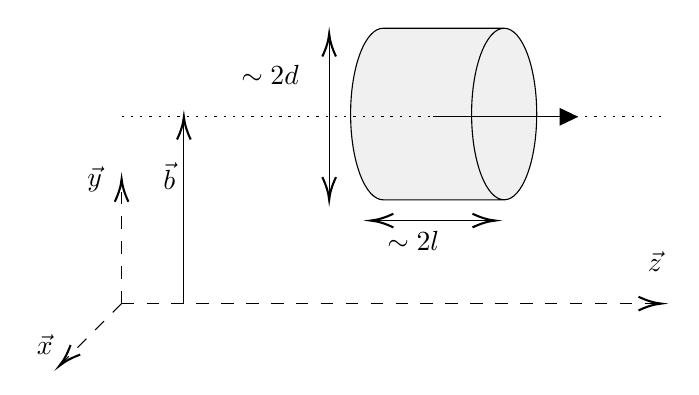
\begin{tikzpicture}[x=0.75pt,y=0.75pt,yscale=-1,xscale=1]
%uncomment if require: \path (0,367); %set diagram left start at 0, and has height of 367

%Flowchart: Direct Access Storage [id:dp8371024262626638] 
\draw  [fill={rgb, 255:red, 240; green, 240; blue, 240 }  ,fill opacity=1 ] (374.31,160) -- (316.03,160) .. controls (307.36,160) and (300.33,141.49) .. (300.33,118.67) .. controls (300.33,95.84) and (307.36,77.33) .. (316.03,77.33) -- (374.31,77.33)(390,118.67) .. controls (390,141.49) and (382.97,160) .. (374.31,160) .. controls (365.64,160) and (358.62,141.49) .. (358.62,118.67) .. controls (358.62,95.84) and (365.64,77.33) .. (374.31,77.33) .. controls (382.97,77.33) and (390,95.84) .. (390,118.67) ;
%Straight Lines [id:da30614936070461374] 
\draw    (312,170) -- (368,170) ;
\draw [shift={(370,170)}, rotate = 180] [color={rgb, 255:red, 0; green, 0; blue, 0 }  ][line width=0.75]    (10.93,-3.29) .. controls (6.95,-1.4) and (3.31,-0.3) .. (0,0) .. controls (3.31,0.3) and (6.95,1.4) .. (10.93,3.29)   ;
\draw [shift={(310,170)}, rotate = 0] [color={rgb, 255:red, 0; green, 0; blue, 0 }  ][line width=0.75]    (10.93,-3.29) .. controls (6.95,-1.4) and (3.31,-0.3) .. (0,0) .. controls (3.31,0.3) and (6.95,1.4) .. (10.93,3.29)   ;
%Straight Lines [id:da9389864851557561] 
\draw    (290,158) -- (290,82) ;
\draw [shift={(290,80)}, rotate = 450] [color={rgb, 255:red, 0; green, 0; blue, 0 }  ][line width=0.75]    (10.93,-3.29) .. controls (6.95,-1.4) and (3.31,-0.3) .. (0,0) .. controls (3.31,0.3) and (6.95,1.4) .. (10.93,3.29)   ;
\draw [shift={(290,160)}, rotate = 270] [color={rgb, 255:red, 0; green, 0; blue, 0 }  ][line width=0.75]    (10.93,-3.29) .. controls (6.95,-1.4) and (3.31,-0.3) .. (0,0) .. controls (3.31,0.3) and (6.95,1.4) .. (10.93,3.29)   ;
%Straight Lines [id:da11405166277620071] 
\draw  [dash pattern={on 4.5pt off 4.5pt}]  (190,210) -- (448,210) ;
\draw [shift={(450,210)}, rotate = 180] [color={rgb, 255:red, 0; green, 0; blue, 0 }  ][line width=0.75]    (10.93,-3.29) .. controls (6.95,-1.4) and (3.31,-0.3) .. (0,0) .. controls (3.31,0.3) and (6.95,1.4) .. (10.93,3.29)   ;

%Straight Lines [id:da28383638822907975] 
\draw    (340,120) -- (408,120) ;
\draw [shift={(410,120)}, rotate = 180] [fill={rgb, 255:red, 0; green, 0; blue, 0 }  ][line width=0.75]  [draw opacity=0] (8.93,-4.29) -- (0,0) -- (8.93,4.29) -- cycle    ;

%Straight Lines [id:da9877009376243533] 
\draw  [dash pattern={on 0.84pt off 2.51pt}]  (190,120) -- (450,120) ;


%Straight Lines [id:da9161183968027347] 
\draw  [dash pattern={on 4.5pt off 4.5pt}]  (190,210) -- (190,152) ;
\draw [shift={(190,150)}, rotate = 450] [color={rgb, 255:red, 0; green, 0; blue, 0 }  ][line width=0.75]    (10.93,-3.29) .. controls (6.95,-1.4) and (3.31,-0.3) .. (0,0) .. controls (3.31,0.3) and (6.95,1.4) .. (10.93,3.29)   ;

%Straight Lines [id:da010683741846586159] 
\draw  [dash pattern={on 4.5pt off 4.5pt}]  (190,210) -- (161.41,238.59) ;
\draw [shift={(160,240)}, rotate = 315] [color={rgb, 255:red, 0; green, 0; blue, 0 }  ][line width=0.75]    (10.93,-3.29) .. controls (6.95,-1.4) and (3.31,-0.3) .. (0,0) .. controls (3.31,0.3) and (6.95,1.4) .. (10.93,3.29)   ;

%Straight Lines [id:da5050884694855691] 
\draw    (220,210) -- (220,122) ;
\draw [shift={(220,120)}, rotate = 450] [color={rgb, 255:red, 0; green, 0; blue, 0 }  ][line width=0.75]    (10.93,-3.29) .. controls (6.95,-1.4) and (3.31,-0.3) .. (0,0) .. controls (3.31,0.3) and (6.95,1.4) .. (10.93,3.29)   ;


% Text Node
\draw (330.5,180) node   {$\sim 2l$};
% Text Node
\draw (261.5,100) node   {$\sim 2d$};
% Text Node
\draw (153,230) node   {$\vec{x}$};
% Text Node
\draw (177,150) node   {$\vec{y}$};
% Text Node
\draw (447,190) node   {$\vec{z}$};
% Text Node
\draw (213,148.5) node   {$\vec{b}$};


\end{tikzpicture}
    \caption{Schema del pacchetto d'onda incidente.}
    \label{fig:pacchettoincidente}
\end{figure}


\subsection{Pacchetto d'onda diffuso}

Il risultato appena trovato {\`e} l'analogo della funzione $e^{\frac{i}{\hbar}  \vec{p} \cdot
\vec{x}}$ di prima, che descriveva il pacchtto molto prima dell'urto, quando
la particella {\`e} libera.

Ora per{\`o} vorremmo anche costruire l'analogo in versione di pacchetto
d'onda della funzione asintotica \eqref{formaasintotica}, che per distinguerla dalla $\psi_{\text{as}}$ la denoteremo con $\psi_{\text{in}}$ (da interazione). Mentre le soluzioni
stazionarie per una particella libera sono note, nel caso di una particella
deviata da un potenziale $V$ non lo sono. Per trovarla imponiamo che tale
funzione obbedisca all'equazione della dinamica $H \psi_{\text{in}} (\vec{x})
= \mathcal{E} \psi_{\text{in}} (\vec{x})$ con l'hamiltoniana $H$ ``vera'',
cio{\`e} quella completa di potenziale di interazione $V (\vec{x})$:
\begin{equation}
  \label{lippmann1} \left( - \frac{\hbar^2}{2 m} \nabla^2 + V (\vec{x})
  \right) \psi_{\text{in}} (\vec{x}) = \frac{p^2}{2 m} \psi_{\text{in}}
  (\vec{x})
\end{equation}
Dobbiamo dinque risolvere questa equazione per trovare la $\psi_{\text{in}}
(\vec{x})$, da cui poi sar{\`a} possibile costruire il pacchetto. Tutto lo
scopo dello scattering {\`e} ricavare da questa analisi la forma di $V
(\vec{x})$ dalla sezione d'urto. Riscriviamo la {\eqref{lippmann1}} in una
forma diversa:
\begin{equation}
  \label{lippmann2} \left( \frac{\hbar^2}{2 m} \nabla^2 + \frac{p^2}{2 m}
  \right) \psi_{\text{in}} (\vec{x}) = V (\vec{x}) \psi_{\text{in}}
\end{equation}
conosciuta come {\tmem{Equazione di Lippmann-Schwinger}}. In questa forma
l'equazione {\`e} pi{\`u} semplice da risolvere per il fatto che la si pu{\`o}
vedere in forma operatoriale come
\[ A_p \psi_{\text{in}} (\vec{x}) = V (\vec{x}) \psi_{\text{in}} (\vec{x})
   \qquad \text{con} \qquad A_p = \frac{\hbar^2}{2 m} \nabla^2 + \frac{p^2}{2
   m} \]
Osserviamo per prima cosa che l'onda piana $e^{\frac{i}{\hbar}  \vec{p} \cdot
\vec{x}}$ soddisfa l'omogenea associata $A_p e^{\frac{i}{\hbar}  \vec{p} \cdot
\vec{x}} = 0$, infatti applicando $\frac{\hbar^2}{2 m} \nabla^2$ a
$e^{\frac{i}{\hbar}  \vec{p} \cdot \vec{x}}$ si ottiene $- \frac{p^2}{2 m}$.
Pertanto $e^{\frac{i}{\hbar}  \vec{p} \cdot \vec{x}}$ {\`e} una soluzione
dell'omogenea associata all'equazione di Lippmann-Schwinger, mentre una
soluzione particolare si pu{\`o} trovare invertendo l'operatore $A_p$:
\[ A_p \psi_{\text{in}} = V \psi_{\text{in}}  \quad \Longrightarrow \quad
   \psi_{\text{in}} = A_p^{- 1} V \psi_{\text{in}} \]
La soluzione formale generale {\`e} la somma della soluzione dell'omogenea
pi{\`u} quella particolare:
\begin{equation}
\label{soluzionegenerale}
\psi_{\text{in}} (\vec{x}) = e^{\frac{i}{\hbar}  \vec{p} \cdot \vec{x}} +
   (A_p^{- 1} V \psi_{\text{in}}) (\vec{x})
\end{equation}
Tale equazione {\`e} implicita (non determina esplicitamente
$\psi_{\text{in}}$), e questo causa alcune complicazioni che vedremo pi{\`u}
avanti. Come vedremo in seguito, il primo termine corrisponde alla funzione
d'onda incidente, mentre il secondo a quella diffusa. La $\psi_{\text{in}}
(\vec{x})$ {\`e} la funzione d'onda stazionaria con $p$ fissato, mentre la
soluzione pi{\`u} generale {\`e} il pacchetto di tutte le $\psi_{\text{in}}
(\vec{x})$ integrate su $p$:
\[ \psi (\vec{x}, t) = \int \frac{d^3 p}{(2 \pi \hbar)^3}  \tilde{g} (\vec{p}
   - \vec{p}_0) \psi_{\text{in}} (\vec{x}) e^{- \frac{i}{\hbar} 
   \frac{\vec{p}^2}{2 m} t} \]
Ora per{\`o} vogliamo scegliere una forma particolare di $A_p^{- 1}$ tale che
per $t \to - \infty$ il termine $A_p^{- 1} V \psi_{\text{in}}$ della \eqref{soluzionegenerale} non dia il
contributo al pacchetto. In questo modo impongo che per $t \to - \infty$ mi
rimanga solo il termine $e^{\frac{i}{\hbar}  \vec{p} \cdot \vec{x}}$. Per far
questo {\`e} per{\`o} necessario invertire l'operatore differenziale $A_p$.
Rappresentiamo innanzitutto $A_p^{- 1}$ in forma integrale, ovvero scrivo
l'azione dell'operatore come un integrale:
\begin{equation}
\label{kerintegrale}
A_p^{- 1} (V \psi_{\text{in}} (\vec{x})) = \int d^3 y \hspace{0.17em}
   A_p^{- 1} (\vec{x} - \vec{y}) V (\vec{y}) \psi_{\text{in}} (\vec{y})
\end{equation}
detto anche \tmtextit{nucleo integrale}. La funzione $A_p^{- 1} (\vec{x} -
\vec{y})$ deve ovviamente soddisfare l'identit{\`a}
\[ A_p A_p^{- 1} (\vec{x} - \vec{y}) = \delta^3 (\vec{x} - \vec{y}) \]
In modo che $A_p^{- 1}$ sia effettivamente l'inverso di $A_p$ anche in forma
integrale. Per trovare un'espressione integrale di $A_p^{- 1} (\vec{x} -
\vec{y})$ si utilizza la trasformata di Fourier:
\[ A_p = \frac{\hbar^2}{2 m}  \vec{\nabla}^2 + \frac{p^2}{2 m} \quad
   \xRightarrow{\text{Fourier}} \quad \tilde{A}_p (\vec{q}) = -
   \frac{\vec{q}^2}{2 m} + \frac{\vec{p}^2}{2 m} \]
Questa, in generale, {\`e} la ``regola d'oro'' per invertire operatori
differenziali: siccome la trasformata di Fourier di operatori differenziali
{\`e} sempre in forma polinomiale, ci{\`o} che si fa {\`e} applicare la
trasformata ottenendo un polinomio, invertire tale polinomio e una volta fatto
ci{\`o} si applica l'antitrasformata per ricavare il nucleo integrale. Ma nel
nostro caso $\tilde{A}_p (\vec{q})$ {\`e} uno scalare, pertanto l'inverso di
$\tilde{A}_p (\vec{q})$ sar{\`a} il suo reciproco:
\[ \widetilde{A_p^{- 1}} (\vec{q}) = \frac{1}{\tilde{A}_p (\vec{q})} =
   \frac{1}{\frac{p^2}{2 m} - \frac{q^2}{2 m}} \]
A questo punto rimarrebbe da invertire questa distribuzione. Tuttavia si ha
una singolarit{\`a} per $| p | = q$, quindi tale oggetto non {\`e} una
distribuzione ben definita, e occorre una regolarizzazione. Ad esempio di
pu{\`o} utilizzare la \tmtextit{parte principale}. Oppure, un altro metodo
efficace di regolarizzazione {\`e} la \tmtextit{prescrizione $\pm i \delta$}:
\[ \widetilde{A_p^{- 1}} (\vec{q}) = \frac{1}{\frac{p^2}{2 m} - \frac{q^2}{2
   m} + i \delta} \qquad (\delta \rightarrow 0) \]
Quindi, applicando la trasformata inversa a quest'ultima espressione si
ottiene
\begin{equation}
\label{inverseA} A_p^{- 1}  (\vec{x} - \vec{y}) = \int \frac{d^3 q}{(2 \pi
   \hbar)^3}  \frac{e^{- i \frac{\vec{q}}{\hbar} \cdot (\vec{x} -
   \vec{y})}}{\frac{p^2}{2 m} - \frac{q^2}{2 m} + i \delta}
\end{equation}
Dimostriamo dunque che il contributo $A_p^{- 1} V \psi_{\text{in}}$ della
soluzione stazionaria (e quindi anche di quello di un qualunque pacchetto
d'onda) dell'equazione di Lippmann-Schwinger tende a zero per $t \to -
\infty$. Inseriamo nella \eqref{kerintegrale} la
forma a pacchetto di $\psi_{\text{in}}$ e la forma \eqref{inverseA} appena ricavata di $A_p^{-
1}$:
\[ (A_p^{- 1} V \psi_{\text{in}}) (\vec{x}) = \int d^3 y \hspace{0.17em}
   A_p^{- 1} (\vec{x} - \vec{y}) V (\vec{y}) \psi_{\text{in}} (\vec{y}) \]
\[ = \int d^3 y \hspace{0.17em} \int \frac{d^3 q}{(2 \pi \hbar)^3}  \frac{e^{-
   i \frac{\vec{q}}{\hbar}  (\vec{x} - \vec{y})}}{\frac{p^2}{2 m} -
   \frac{q^2}{2 m} + i \delta} V (\vec{y})  \int \frac{d^3 p}{(2 \pi \hbar)^3}
   \underbrace{\tilde{g} (\vec{p} - \vec{p}_0)}_{\tilde{g}_{\vec{p}_0}
   (\vec{p})_{}} e^{\frac{i}{\hbar}  \vec{p} \cdot (\vec{y} - \vec{b})} e^{-
   \frac{i}{\hbar}  \frac{p^2}{2 m} t} \]
dove la $\psi_{\text{in}}$ {\`e} sata scritta come un pacchetto di onde piane,
ovvero la soluzione dell'omogenea associata dell'equazione di
Lippman-Schwinger (shiftata in $\vec{x}$ del parametro d'impatto $\vec{b}$).
L'ultima espressione la possiamo riscrivere riarrangiando i termini
all'interno degli integrali, come
\[ (A_p^{- 1} V \psi_{\text{in}}) (\vec{x}) = \int d^3 yV (\vec{y}) \hspace{0.17em} \int \frac{d^3 q}{(2 \pi \hbar)^3}
   e^{- i \frac{\vec{q}}{\hbar}  (\vec{x} - \vec{y})}  \int \frac{d^3 p}{(2
   \pi \hbar)^3}  \tilde{g}_{\vec{p}_0} (\vec{p}) \frac{e^{\frac{i}{\hbar} 
   \vec{p} \cdot (\vec{y} - \vec{b})} e^{- \frac{i}{\hbar}  \frac{p^2}{2 m}
   t}}{\frac{p^2}{2 m} - \frac{q^2}{2 m} + i \delta} \]
A questo punto dimostriamo che il terzo integrale
\begin{equation}
  \label{integraledelta} \int \frac{d^3 p}{(2 \pi \hbar)^3} 
  \tilde{g}_{\vec{p}_0} (\vec{p}) \frac{e^{\frac{i}{\hbar}  \vec{p} \cdot
  (\vec{y} - \vec{b})} e^{- \frac{i}{\hbar}  \frac{p^2}{2 m} t}}{\frac{p^2}{2
  m} - \frac{q^2}{2 m} + i \delta}
\end{equation}
{\`e} nullo per $t \rightarrow - \infty$. Per farlo dobbiamo calcolare
l'integrale scrivendo la $\tilde{g}_{\vec{p}_0} (\vec{p})$ in coordinate
polari $(| \vec{p} |, \theta_p, \varphi_p)$ lungo l'asse $\vec{x} - \vec{b}$
ed eseguendo un cambio di variabile $p \to \mathcal{E}= \frac{p^2}{2 m}$.
Indicando con $d \Omega_p$ l'angolo solido in $p$ si ottiene
\begin{eqnarray*}
  d^3 p & \rightarrow & p^2 d p \overbrace{d \theta_p d \varphi_p}^{d
  \Omega_p}\\
  & = & 2 m E d \left( \sqrt{2 m E} \right) d \Omega_p\\
  & = & 2 m E  \sqrt{2 m}  \frac{1}{2 \sqrt{E}} d E d \Omega_p\\
  & = & \frac{(2 m)^{\frac{3}{2}}}{2} \sqrt{\mathcal{E}} d\mathcal{E}d
  \Omega_p
\end{eqnarray*}
\[ \tilde{g} (\vec{p}) = \tilde{g} (| \vec{p} |, \theta_p, \varphi_p) =
   \tilde{g} (\sqrt{2 m\mathcal{E}}, \theta_p, \varphi_p) \]
L'integrale {\eqref{integraledelta}} diventa quindi
\[ \frac{(2 m)^{\frac{3}{2}}}{2}  \int \frac{d \Omega_p}{(2 \pi \hbar)^3} 
   \int_{- \infty}^{+ \infty} d\mathcal{E} \sqrt{\mathcal{E}} H (\mathcal{E})
   \tilde{g} (\sqrt{2 m\mathcal{E}}, \theta_p, \varphi_p)
   \frac{e^{\frac{i}{\hbar} \sqrt{2 m\mathcal{E}} | \vec{x} - \vec{b} | \cos
   \theta_p} e^{- \frac{i}{\hbar} E t} }{\mathcal{E}- \left( \frac{q^2}{2 m} -
   i \delta \right)} \]
dove $H$ {\`e} la funzione di Heaviside (l'integrale in $E$ senza la $H$
andrebbe da $0$ a $+ \infty$). Usando il teorema dei residui, poich{\'e} il
polo si trova in $\mathcal{E}= \frac{q^2}{2 m} - i \delta$, per $t < 0$ in
modulo sufficientemente grande possiamo chiudere il contorno nel semipiano
complesso Im$\mathcal{E}> 0$:

\begin{center}


\tikzset{every picture/.style={line width=0.75pt}} %set default line width to 0.75pt        

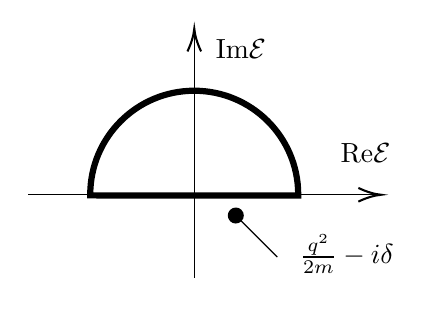
\begin{tikzpicture}[x=0.75pt,y=0.75pt,yscale=-1,xscale=1]
%uncomment if require: \path (0,213); %set diagram left start at 0, and has height of 213

%Straight Lines [id:da5450173168058778] 
\draw    (320,160) -- (320,42) ;
\draw [shift={(320,40)}, rotate = 450] [color={rgb, 255:red, 0; green, 0; blue, 0 }  ][line width=0.75]    (10.93,-3.29) .. controls (6.95,-1.4) and (3.31,-0.3) .. (0,0) .. controls (3.31,0.3) and (6.95,1.4) .. (10.93,3.29)   ;

%Straight Lines [id:da831200302130011] 
\draw    (240,120) -- (408,120) ;
\draw [shift={(410,120)}, rotate = 180] [color={rgb, 255:red, 0; green, 0; blue, 0 }  ][line width=0.75]    (10.93,-3.29) .. controls (6.95,-1.4) and (3.31,-0.3) .. (0,0) .. controls (3.31,0.3) and (6.95,1.4) .. (10.93,3.29)   ;

%Shape: Chord [id:dp4506491533130468] 
\draw  [color={rgb, 255:red, 0; green, 0; blue, 0 }  ,draw opacity=1 ][line width=2.25]  (269.88,120.3) .. controls (269.88,120.2) and (269.88,120.1) .. (269.88,120) .. controls (269.81,92.39) and (292.19,69.95) .. (319.85,69.88) .. controls (347.52,69.81) and (370.01,92.14) .. (370.07,119.76) .. controls (370.07,119.95) and (370.07,120.15) .. (370.07,120.35) -- cycle ;
%Straight Lines [id:da681775789324145] 
\draw [color={rgb, 255:red, 0; green, 0; blue, 0 }  ,draw opacity=1 ][fill={rgb, 255:red, 136; green, 136; blue, 136 }  ,fill opacity=1 ]   (340,130) -- (360,150) ;

\draw [shift={(340,130)}, rotate = 45] [color={rgb, 255:red, 0; green, 0; blue, 0 }  ,draw opacity=1 ][fill={rgb, 255:red, 0; green, 0; blue, 0 }  ,fill opacity=1 ][line width=0.75]      (0, 0) circle [x radius= 3.35, y radius= 3.35]   ;
%Straight Lines [id:da4476031967934708] 
\draw    (340,130) ;



% Text Node
\draw (393.5,148.5) node   {$\frac{q^{2}}{2m} -i\delta $};
% Text Node
\draw (342.5,50) node   {$\mathrm{Im}\mathcal{E}$};
% Text Node
\draw (402.5,100) node   {$\mathrm{Re}\mathcal{E}$};

\end{tikzpicture}
\end{center}

Per $t \to - \infty$ domina il termine $e^{- \frac{i}{\hbar} E t}$. L'area
scelta non contiene poli pertanto l'integrale {\`e} pari a zero, e cos{\`i} a
$t \to - \infty$ il termine $A_p^{- 1} V \psi_{\text{in}}$ {\`e} nullo e non
contribuisce al pacchetto.

Rimane ora da mostrare che per $t \to + \infty$ il termine $A_p^{- 1} V
\psi_{\text{in}}$ {\tmem{riproduce un pacchetto diffuso}} e che
\tmtextit{determina $f$ in funzione di $V$}. Poniamoci innanzitutto
nell'approssimazione $D \gg a, \Delta x$. Riscriviamo la {\eqref{inverseA}}
come
\begin{eqnarray*}
  A_p^{- 1}  (\vec{x} - \vec{y}) & = & \int \frac{d^3 q}{(2 \pi \hbar)^3} 
  \frac{e^{\frac{i}{\hbar} \vec{q} \cdot (\vec{x} -
  \vec{y})}}{\frac{\vec{p}^2}{2 m} - \frac{\vec{q}^2}{2 m} + i \delta}\\
  & = & 2 m \int \frac{d^3 q}{(2 \pi \hbar)^3}  \frac{e^{\frac{i}{\hbar}
  \vec{q} \cdot (\vec{x} - \vec{y})}}{p^2 - q^2 + im \delta}\\
  & = & \frac{2 m}{(2 \pi \hbar)^3} \int d^3 q \frac{e^{\frac{i}{\hbar}
  \vec{q} \cdot (\vec{x} - \vec{y})}}{p^2 - q^2 + i \delta}
\end{eqnarray*}
dove nell'ultimo passaggio si {\`e} operata la sostituzone $m \delta
\rightarrow \delta$ dato che rappresenta comunque un termine che deve tendere
a $0$. Passando poi in coordinate polari $(| \vec{q} |, \theta_q, \varphi_q)$
si ottiene (ricordando lo jacobiano $q^2$):
\begingroup
\allowdisplaybreaks
\begin{eqnarray*}
  A_p^{- 1}  (\vec{x} - \vec{y}) & = & \frac{2 m}{(2 \pi \hbar)^3}  \underbrace{\int_0^{2 \pi} d
  \varphi_q}_{2 \pi}  \int_{- 1}^1 d \cos \theta_q  \int_0^{+ \infty} d q
  \frac{e^{\frac{i}{\hbar} q | \vec{x} - \vec{y} | \cos \theta_q}}{p^2 - q^2 +
  i \delta} q^2\\
  & = & \frac{2 m}{\hbar^3}  \frac{1}{(2 \pi)^2}  \int_{- 1}^1 d k \int_0^{+
  \infty} d q \frac{e^{\frac{i}{\hbar} q | \vec{x} - \vec{y} | k}}{p^2 - q^2 +
  i \delta} q^2 \qquad (k = \cos \theta_q)\\
  & = & \frac{2 m}{\hbar^3}  \frac{1}{(2 \pi)^2} \int_0^{+ \infty} d q
  \frac{\hbar}{i}  \frac{q^2 }{q | \vec{x} - \vec{y} |} 
  \frac{e^{\frac{i}{\hbar} q | \vec{x} - \vec{y} |} - e^{- \frac{i}{\hbar} q |
  \vec{x} - \vec{y} |}}{p^2 - q^2 + i \delta}\\
  & = & i \frac{2 m}{(2 \pi \hbar)^2}  \frac{1}{| \vec{x} - \vec{y} |}
  \int_0^{+ \infty} d q \frac{q e^{\frac{i}{\hbar} q | \vec{x} - \vec{y} |} -
  q e^{- \frac{i}{\hbar} q | \vec{x} - \vec{y} |}}{p^2 - q^2 + i \delta}\\
  & = & i \frac{2 m}{(2 \pi \hbar)^2}  \frac{1}{| \vec{x} - \vec{y} |} \left(
  \int_0^{+ \infty} d q \frac{q e^{\frac{i}{\hbar} q | \vec{x} - \vec{y}
  |}}{p^2 - q^2 + i \delta} - \int_0^{+ \infty} d q \frac{q e^{-
  \frac{i}{\hbar} q | \vec{x} - \vec{y} |}}{p^2 - q^2 + i \delta} \right)\\
  & = & i \frac{2 m}{(2 \pi \hbar)^2}  \frac{1}{| \vec{x} - \vec{y} |} \left(
  \int_0^{+ \infty} d q \frac{q e^{\frac{i}{\hbar} q | \vec{x} - \vec{y}
  |}}{p^2 - q^2 + i \delta} + \underbrace{\int^0_{- \infty} d^{} q \frac{q
  e^{+ \frac{i}{\hbar} q | \vec{x} - \vec{y} |}}{p^2 - q^2 + i \delta}}_{q
  \rightarrow - q} \right)\\
  & = & i \frac{2 m}{(2 \pi \hbar)^2 | \vec{x} - \vec{y} |}  \int_{-
  \infty}^{+ \infty} d q \frac{q}{q^2 - p^2 - i \delta} e^{\frac{i}{\hbar} q |
  \vec{x} - \vec{y} |}
\end{eqnarray*}
\endgroup
Si hanno dunque due poli in $\pm \sqrt{p^2 + i \delta}$, che posso espandere
in $\pm (p + i \delta)$ per $\delta \rightarrow 0$. Chiudiamo il contorno per
$\mathrm{Im} q > 0$:


\begin{center}
\tikzset{every picture/.style={line width=0.75pt}} %set default line width to 0.75pt        

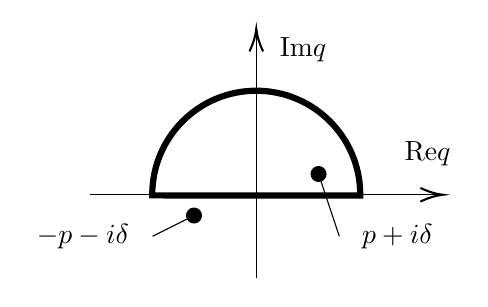
\begin{tikzpicture}[x=0.75pt,y=0.75pt,yscale=-1,xscale=1]
%uncomment if require: \path (0,213); %set diagram left start at 0, and has height of 213

%Straight Lines [id:da4342137218095983] 
\draw    (320,160) -- (320,42) ;
\draw [shift={(320,40)}, rotate = 450] [color={rgb, 255:red, 0; green, 0; blue, 0 }  ][line width=0.75]    (10.93,-3.29) .. controls (6.95,-1.4) and (3.31,-0.3) .. (0,0) .. controls (3.31,0.3) and (6.95,1.4) .. (10.93,3.29)   ;

%Straight Lines [id:da4251379954059913] 
\draw    (240,120) -- (408,120) ;
\draw [shift={(410,120)}, rotate = 180] [color={rgb, 255:red, 0; green, 0; blue, 0 }  ][line width=0.75]    (10.93,-3.29) .. controls (6.95,-1.4) and (3.31,-0.3) .. (0,0) .. controls (3.31,0.3) and (6.95,1.4) .. (10.93,3.29)   ;

%Shape: Chord [id:dp9771682085205091] 
\draw  [color={rgb, 255:red, 0; green, 0; blue, 0 }  ,draw opacity=1 ][line width=2.25]  (269.88,120.3) .. controls (269.88,120.2) and (269.88,120.1) .. (269.88,120) .. controls (269.81,92.39) and (292.19,69.95) .. (319.85,69.88) .. controls (347.52,69.81) and (370.01,92.14) .. (370.07,119.76) .. controls (370.07,119.95) and (370.07,120.15) .. (370.07,120.35) -- cycle ;
%Straight Lines [id:da2846806342017081] 
\draw [color={rgb, 255:red, 0; green, 0; blue, 0 }  ,draw opacity=1 ][fill={rgb, 255:red, 136; green, 136; blue, 136 }  ,fill opacity=1 ]   (350,110) -- (360,140) ;

\draw [shift={(350,110)}, rotate = 71.57] [color={rgb, 255:red, 0; green, 0; blue, 0 }  ,draw opacity=1 ][fill={rgb, 255:red, 0; green, 0; blue, 0 }  ,fill opacity=1 ][line width=0.75]      (0, 0) circle [x radius= 3.35, y radius= 3.35]   ;
%Straight Lines [id:da40121448843342056] 
\draw    (340,130) ;


%Straight Lines [id:da8339030663676579] 
\draw [color={rgb, 255:red, 0; green, 0; blue, 0 }  ,draw opacity=1 ][fill={rgb, 255:red, 136; green, 136; blue, 136 }  ,fill opacity=1 ]   (290,130) -- (270,140) ;

\draw [shift={(290,130)}, rotate = 153.43] [color={rgb, 255:red, 0; green, 0; blue, 0 }  ,draw opacity=1 ][fill={rgb, 255:red, 0; green, 0; blue, 0 }  ,fill opacity=1 ][line width=0.75]      (0, 0) circle [x radius= 3.35, y radius= 3.35]   ;

% Text Node
\draw (388,140) node   {$p+i\delta $};
% Text Node
\draw (342.5,50) node   {$\mathrm{Im} q$};
% Text Node
\draw (402.5,100) node   {$\mathrm{Re} q$};
% Text Node
\draw (236.5,140) node   {$-p-i\delta $};

\end{tikzpicture}
\end{center}


Utilizzando il teorema dei residui si ottiene infine
\begin{eqnarray*}
  A_p^{- 1}  (\vec{x} - \vec{y}) & = & i \frac{2 m}{(2 \pi \hbar)^2 | \vec{x}
  - \vec{y} |}  \int_{- \infty}^{+ \infty} d q \frac{q}{q^2 - p^2 - i \delta}
  e^{\frac{i}{\hbar} q | \vec{x} - \vec{y} |}\\
  & = & i \frac{2 m}{(2 \pi \hbar)^2 | \vec{x} - \vec{y} |} 2 \pi i
  \frac{p}{2 p} e^{\frac{i}{\hbar} p | \vec{x} - \vec{y} |}\\
  & = & - \frac{2 m}{\hbar^2}  \frac{1}{4 \pi}  \frac{e^{\frac{i}{\hbar} p | \vec{x} -
  \vec{y} |}}{| \vec{x} - \vec{y} |}
\end{eqnarray*}
Il potenziale $V$ {\`e} non nullo solo vicino al centro diffusore. La
$\vec{y}$ {\`e} integrata sul supporto del potenziale $V (\vec{y})$, ovvero
nei punti vicino all'origine, cio{\`e} per $| \vec{y} | \lesssim a$.
Nell'equazione di Lippmann-Schwinger abbiamo dunque che $A_p^{- 1}  (\vec{x} -
\vec{y}) V (\vec{y}) \psi_{\text{in}} (\vec{y}) \neq 0$ solo per $| \vec{y} |
\lesssim a \ll D = | \vec{x} |$.

Si ha poi che $| \vec{x} | \sim D$, e dato che ci poniamo nell'approssimazione
$a \ll D$, quindi $| \vec{y} | \ll | \vec{x} |$ si pu{\`o} espandere $|
\vec{x} - \vec{y} |$ ottenendo
\[ | \vec{x} - \vec{y} | = \sqrt{x^2 + y^2 - 2 \vec{x} \cdot \vec{y}} \simeq |
   \vec{x} | \left( 1 - \frac{1}{2} \cdot 2 \frac{\vec{x} \cdot \vec{y}}{x^2}
   \right) = | \vec{x} | - \hat{r} \cdot \vec{y} = r - \hat{r} \cdot \vec{y}
\]
in cui abbiamo posto $| \vec{x} | = r$, e da questo si ottiene
\begin{align}
  A_p^{- 1}  (\vec{x} - \vec{y}) & = - \frac{2 m}{\hbar^2}  \frac{1}{4 \pi} 
  \frac{e^{\frac{i}{\hbar} p | \vec{x} - \vec{y} |}}{| \vec{x} - \vec{y} |} \notag \\
  & \simeq - \frac{2 m}{\hbar^2}  \frac{1}{4 \pi}  \frac{e^{\frac{i}{\hbar} p (r -
  \hat{r} \cdot \vec{y})}}{r - \underbrace{\hat{r} \cdot \vec{y}}_{\ll r}} \notag \\
  & \simeq - \frac{2 m}{\hbar^2}  \frac{1}{4 \pi}  \frac{e^{\frac{i}{\hbar} pr}}{r} e^{-
  \frac{i}{\hbar} p \hat{r} \cdot \vec{y}} \label{approssimazioneInvA}
\end{align}
A questo punto consideriamo il pacchetto $\psi_d (\vec{x}, t)$ costituito
dalle soluzioni stazionarie $A_p^{- 1} V \psi_{\text{in}}$ relative alla
componente diffusa:
\[ \psi_d (\vec{x}, t) = \int \frac{d^3 p}{(2 \pi \hbar)^3}  \tilde{g}
   (\vec{p} - \vec{p}_0) e^{- \frac{i}{\hbar} \vec{p} \cdot \vec{b}} e^{-
   \frac{i}{\hbar} \frac{p^2}{2 m} t} (A_p^{- 1} V \psi_{\text{in}}) (\vec{x})
\]
dove si {\`e} inserito anche lo shift di $\vec{b}$ e il termine di evoluzione
temporale.

A questo punto si inserisce nell'equazione precedente la forma integrale \eqref{kerintegrale} di $A_p^{- 1} V \psi_{\text{in}}$:
\[ \psi_d (\vec{x}, t) = \int \frac{d^3 p}{(2 \pi \hbar)^3} 
   \tilde{g}_{\vec{p}_0} (\vec{p}) e^{- \frac{i}{\hbar} \vec{p} \cdot \vec{b}}
   e^{- \frac{i}{\hbar} \frac{p^2}{2 m} t} \int d^3 y \hspace{0.17em} A_p^{-
   1} (\vec{x} - \vec{y}) V (\vec{y}) \psi_{\text{in}} (\vec{y}) \]
e si inserisce poi l'approssimazione \eqref{approssimazioneInvA} di $A_p^{- 1}  (\vec{x} - \vec{y})$
all'interno del pacchetto ottenendo
\[ \psi_d (\vec{x}, t) = \int \frac{d^3 p}{(2 \pi \hbar)^3}  \tilde{g}_{\vec{p}_0} (\vec{p}) e^{-
   \frac{i}{\hbar} \vec{p} \cdot \vec{b}} e^{- \frac{i}{\hbar} \frac{p^2}{2 m}
   t} \int d^3 y \hspace{0.17em} \left( - \frac{2 m}{\hbar^2}  \frac{1}{4 \pi}
   \frac{e^{\frac{i}{\hbar} pr}}{r} e^{- \frac{i}{\hbar} p \hat{r} \cdot
   \vec{y}} \right) V (\vec{y}) \psi_{\text{in}} (\vec{y}) \]
Si possono isolare nell'integrale finale i termini che dipendono da $(\theta,
\varphi)$:
\begin{equation}
\label{eqformaperf}
\psi_d (\vec{x}, t) = \int \frac{d^3 p}{(2 \pi \hbar)^3}  \tilde{g}_{\vec{p}_0} (\vec{p}) e^{-
   \frac{i}{\hbar} \vec{p} \cdot \vec{b}} e^{- \frac{i}{\hbar} \frac{p^2}{2 m}
   t}  \frac{e^{\frac{i}{\hbar} pr}}{r} \underbrace{\int d^3 y \hspace{0.17em}
   \left( - \frac{2 m}{\hbar^2}  \frac{1}{4 \pi} \right) e^{- \frac{i}{\hbar}
   p \hat{r} (\theta, \varphi) \cdot \vec{y}} V (\vec{y}) \psi_{\text{in}}
   (\vec{y})}_{\equiv f_{\vec{p}} (\theta, \varphi)}
\end{equation}
Il termine finale corrisponde alla funzione angolare $f_{\vec{p}} (\theta,
\varphi)$ che avevamo scritto all'inizio della trattazione sullo scattering.
Si ottiene quindi
\begin{equation}
\label{pacchettof}
\psi_d (\vec{x}, t) = \int \frac{d^3 p}{(2 \pi \hbar)^3}  \tilde{g}
   (\vec{p} - \vec{p}_0) e^{- \frac{i}{\hbar} \vec{p} \cdot \vec{b}} e^{-
   \frac{i}{\hbar} \frac{p^2}{2 m} t}  \frac{e^{\frac{i}{\hbar} pr}}{r}
   f_{\vec{p}} (\theta, \varphi)
\end{equation}
A questo punto, esattamente come si è fatto per il pacchetto incidente, si espande in $\vec{p}_0$ (considerando quindi $p \ll p_0$) e
si attua il cambio di variabile $\vec{p} \to \vec{p} + \vec{p}_0$.
Facciamolo per ogni termine:
\begingroup
\allowdisplaybreaks
\begin{eqnarray*}
  \tilde{g} (\vec{p} - \vec{p}_0) & \xrightarrow{\vec{p} \to \vec{p} +
  \overrightarrow{p_0}} & \tilde{g} (\vec{p})
\end{eqnarray*}
\begin{eqnarray*}
  - \frac{i}{\hbar} \vec{p} \cdot \vec{b} & \xrightarrow{\vec{p} \to \vec{p} +
  \overrightarrow{p_0}} & - \frac{i}{\hbar} (\vec{p} + \overrightarrow{p_0})
  \cdot \vec{b}\\
  & = & - \frac{i}{\hbar} (\vec{p} \cdot \vec{b} + \overrightarrow{p_0} \cdot
  \vec{b})\\
  & = & - \frac{i}{\hbar} \vec{p} \cdot \vec{b} \qquad (\overrightarrow{p_0}
  \cdot \vec{b} = 0)
\end{eqnarray*}
\[ \begin{array}{lll}
     - \frac{i}{\hbar} \frac{\vec{p}^2}{2 m} t & \xrightarrow{\vec{p} \to
     \vec{p} + \overrightarrow{p_0}} & - \frac{i}{\hbar}  \frac{(\vec{p} +
     \overrightarrow{p_0}) \cdot (\vec{p} + \overrightarrow{p_0})}{2 m} t\\
     & = & - \frac{i}{\hbar}  \frac{p^2 + p_0^2 + 2 \vec{p} \cdot
     \vec{p}_0}{2 m} t\\
     (p^2 \sim 0) & = & - \frac{i}{\hbar}  \frac{p_0^2}{2 m} t -
     \frac{i}{\hbar}  \frac{\vec{p} \cdot \vec{p}_0}{m} t\\
     &  & - \frac{i}{\hbar}  \frac{p_0^2}{2 m} t - \frac{i}{\hbar}  (\vec{p}
     \cdot \hat{p}_0) \frac{p_0 t}{m}
   \end{array} \]
\[ \begin{array}{lll}
     \frac{i}{\hbar} pr & = & \frac{i}{\hbar}  \sqrt{\vec{p} \cdot \vec{p}}
     r\\
     & \xrightarrow{\vec{p} \to \vec{p} + \overrightarrow{p_0}} &
     \frac{i}{\hbar}  \sqrt{(\vec{p} + \overrightarrow{p_0}) \cdot (\vec{p} +
     \overrightarrow{p_0})} r\\
     & = & \frac{i}{\hbar}  \sqrt{p^2 + p_0^2 + 2 \vec{p}_0 \cdot \vec{p}}
     r\\
     (p^2 \sim 0) & = & \frac{i}{\hbar}  \sqrt{p_0^2 + 2 \vec{p}_0 \cdot
     \vec{p}} r\\
     & = & \frac{i}{\hbar} p_0 \sqrt{1 + 2 \hat{p}_0 \cdot
     \frac{\vec{p}}{p_0}} r\\
     & \simeq & \frac{i}{\hbar} p_0 \left( 1 + \hat{p}_0 \cdot
     \frac{\vec{p}}{p_0} \right) r\\
     & = & \frac{i}{\hbar} p_0 r + \frac{i}{\hbar}  \hat{p}_0 \cdot \vec{p} r
   \end{array} \]
\begin{eqnarray*}
  f_{\vec{p}} (\theta, \varphi) & \xrightarrow{\vec{p} \to \vec{p} +
  \overrightarrow{p_0}} & f_{\vec{p} + \overrightarrow{p_0}} (\theta,
  \varphi)\\
  & = & | f_{\vec{p} + \vec{p}_0} (\theta, \varphi) | e^{i \arg f_{\vec{p} +
  \vec{p}_0}}\\
  & \simeq & | f_{\vec{p}_0} (\theta, \varphi) | e^{i \mathrm{arg} f_{p_0} +
  i \left( \nabla_p \mathrm{arg} f_p \right) |_{p_0} \nobracket \cdot
  \vec{p}}\\
  & = & | f_{\vec{p}_0} (\theta, \varphi) | e^{i \mathrm{arg} f_{p_0} +
  \frac{i}{\hbar}  \overbrace{\hbar \left( \nabla_p \mathrm{arg} f_p \right)
  |_{p_0} \nobracket}^{\equiv \vec{s}} \cdot \vec{p}_{}}\\
  & = & | f_{\vec{p}_0} (\theta, \varphi) | e^{i \mathrm{arg} f_{p_0} +
  \frac{i}{\hbar} \vec{s} \cdot \vec{p}}\\
  & = & | f_{\vec{p}_0} (\theta, \varphi) | e^{i \mathrm{arg} f_{p_0}}
  e^{\frac{i}{\hbar} \vec{s} \cdot \vec{p}}\\
  & = & f_{\vec{p}_0} (\theta, \varphi) e^{\frac{i}{\hbar} \vec{s} \cdot
  \vec{p}}
\end{eqnarray*}
\endgroup
dove si {\`e} definito
\[ \vec{s} \equiv \hbar \left( \nabla_p \mathrm{arg} f_p \right) |_{p_0}
   \nobracket \cdot \vec{p}_0 \]
e vale $| \vec{s} | \simeq a \ll l, d$. Pertanto operando le sostituzioni appena viste nella \eqref{pacchettof} si ottiene
\begingroup
\allowdisplaybreaks
\begin{eqnarray*}
  \psi_d (\vec{x}, t) & = & \int \frac{d^3 p}{(2 \pi \hbar)^3}  \tilde{g}
  (\vec{p}) e^{- \frac{i}{\hbar} \vec{p} \cdot \vec{b}} e^{- \frac{i}{\hbar} 
  \frac{p_0^2}{2 m} t - \frac{i}{\hbar}  (\vec{p} \cdot \hat{p}_0) \frac{p_0
  t}{m}}  \frac{e^{\frac{i}{\hbar} p_0 r + \frac{i}{\hbar}  \hat{p}_0 \cdot
  \vec{p} r}}{r}  f_{\vec{p}_0} (\theta, \varphi) e^{\frac{i}{\hbar} \vec{s}
  \cdot \vec{p}}\\
  & = & \frac{e^{\frac{i}{\hbar} p_0 r}}{r} \int \frac{d^3 p}{(2 \pi
  \hbar)^3}  \tilde{g} (\vec{p}) e^{- \frac{i}{\hbar} \vec{p} \cdot \vec{b}}
  e^{- \frac{i}{\hbar}  (\vec{p} \cdot \hat{p}_0) \frac{p_0 t}{m}}
  e^{\frac{i}{\hbar}  \hat{p}_0 \cdot \vec{p} r} e^{\frac{i}{\hbar} \vec{s}
  \cdot \vec{p}} f_{\vec{p}_0} (\theta, \varphi) e^{- \frac{i}{\hbar} 
  \frac{p_0^2}{2 m} t}\\
  & = & \frac{e^{\frac{i}{\hbar} p_0 r}}{r} \int \frac{d^3 p}{(2 \pi
  \hbar)^3}  \tilde{g} (\vec{p}) e^{- \frac{i}{\hbar} \vec{p} \cdot \vec{b} -
  \frac{i}{\hbar}  (\vec{p} \cdot \hat{p}_0) \frac{p_0 t}{m} + \frac{i}{\hbar}
  \hat{p}_0 \cdot \vec{p} r + \frac{i}{\hbar} \vec{s} \cdot \vec{p}} 
  f_{\vec{p}_0} (\theta, \varphi) e^{- \frac{i}{\hbar}  \frac{p_0^2}{2 m} t}\\
  & = & \frac{e^{\frac{i}{\hbar} p_0 r}}{r} \int \frac{d^3 p}{(2 \pi
  \hbar)^3}  \tilde{g} (\vec{p}) e^{\frac{i}{\hbar} \vec{p} \cdot \left(
  \hat{p}_0  \left( r - \frac{p_0 t}{m} \right) - \vec{b} + \vec{s} \right)} 
  f_{\vec{p}_0} (\theta, \varphi) e^{- \frac{i}{\hbar}  \frac{p_0^2}{2 m} t}\\
  & = & \frac{e^{\frac{i}{\hbar} p_0 r}}{r} g \left( \hat{p}_0  \left( r -
  \frac{p_0 t}{m} \right) - \vec{b} + \vec{s} \right)  f_{\vec{p}_0} (\theta,
  \varphi) e^{- \frac{i}{\hbar}  \frac{p_0^2}{2 m} t}
\end{eqnarray*}
\endgroup

Pertanto la forma finale del pacchetto d'onda diffuso risulta
\begin{equation}
\label{pacchettodiffuso}
\psi_d(\vec x, t) = \frac{e^{\frac{i}{\hbar} p_0 r}}{r} g \left( \hat{p}_0  \left( r -
  \frac{p_0 t}{m} \right) - \vec{b} + \vec{s} \right)  f_{\vec{p}_0} (\theta,
  \varphi) e^{- \frac{i}{\hbar}  \frac{p_0^2}{2 m} t}
\end{equation}

Dalla definizione si ha che il valore del pacchetto {\`e} non trascurabile
solo se $| \vec{b} | \lesssim l$ e $\left| r - \frac{p_0}{m} t \right|
\lesssim d$.



\subsection{Approssimazione di Born per la sezione d'urto}

A questo punto si calcola il modulo quadro della funzione
d'onda \eqref{pacchettodiffuso} del pacchetto diffuso:
\begin{eqnarray*}
  | \psi_d (\vec{x}, t) |^2 & = & \frac{\left| e^{\frac{i}{\hbar} p_0 r}
  \right|^2}{r^2}  \left| g \left( \hat{p}_0  \left( r - \frac{p_0 t}{m}
  \right) - \vec{b} + \vec{s} \right) \right|^2 | f_{\vec{p}_0} (\theta,
  \varphi) |^2 \left| e^{- i \frac{p_0^2}{2 m}  \frac{t}{\hbar}} \right|^2\\
  & = & \frac{1}{r^2}  \left| g \left( \hat{p}_0  \left( r - \frac{p_0 t}{m}
  \right) - \vec{b} + \vec{s} \right) \right|^2 | f_{\vec{p}_0} (\theta,
  \varphi) |^2
\end{eqnarray*}
Si pu{\`o} quindi calcolare la probabilit{\`a} che la particella venga diffusa
nell'unit{\`a} di angolo solido lungo $(\theta, \varphi)$ come
\begin{eqnarray*}
  \Pr (\theta, \varphi) & = & \int d^2 b \int_0^{+ \infty} d^{} r
  \hspace{0.17em} r^2  | \psi_d (\vec{x}, t) |^2\\
  & = & \int d^2 b \int_0^{+ \infty} d^{} r \hspace{0.17em} r^2  | \psi_d (r,
  \theta, \varphi, t) |^2\\
  & = & \int d^2 b \int_0^{+ \infty} \left| g \left( \hat{p}_0  \left( r -
  \frac{p_0}{m} t \right) - \vec{b} + \vec{s} \right) \right|^2  |
  f_{\vec{p}_0} (\theta, \varphi) |^2 \hspace{0.17em} d^{} r
\end{eqnarray*}
Tale probabilit{\`a} ci interessa per il limite di $t \to + \infty$ e per $r$
tra $0$ e $+ \infty$. Si esegue dunque un cambio di varabile $u = r -
\frac{p_0}{m} t$, con $u \in] - \infty, + \infty [$, ottenendo
\begin{eqnarray*}
  \Pr (\theta, \varphi) & = & \int d^2 b \int_{- \infty}^{+ \infty} d^{} u | g
  (\hat{p}_0 u - \vec{b} + \vec{s}) |^2 | f_{\vec{p}_0} (\theta, \varphi)
  |^2\\
  (\vec{p}_0 \perp \vec{b}, \vec{s}) & = & \int d^3 \vec{x}  | g (\vec{x}) |^2
  | f_{\vec{p}_0} (\theta, \varphi) |^2\\
  & = & \| g \|^2  | f_{\vec{p}_0} (\theta, \varphi) |^2
\end{eqnarray*}
Il secondo passaggio {\`e} dato dal fatto che integrare su  $\hat{p}_0 u - \vec{b}
+ \vec{s}$ con $u$ e $\vec{b}$ che variano sui loro domini equivale ad
integrare su $\mathbb{R}^3$. Infatti $\vec{b} + \vec{s}$ varia sul piano
perpendicolare a $\vec{p}_0$ (cio{\`e} su $\mathbb{R}^2$) al variare di
$\vec{b}$, mentre $\hat{p}_0 u$ varia sulla retta generata da $\hat{p}_0$
(cio{\`e} su $\mathbb{R}$) perpendicolare a $\vec{b}$.

La probabilit{\`a} che la particella incida risulta invece (attuando lo stesso
cambio di variabile, ma con $z$ al posto di $r$):
\begingroup
\allowdisplaybreaks
\begin{eqnarray*}
  \text{Pr}_{\text{inc}} & = & \int d^2 b \int_{- \infty}^0 d^{} z \hspace{0.17em} |
  \psi_i (\vec{x}, t) |^2\\
  & = & \int d^2 b \int_{- \infty}^0 d^{} z \hspace{0.17em} | \psi_i (0, 0,
  z, t) |^2\\
  & = & \int d^2 b \int_{- \infty}^0 d^{} z \hspace{0.17em} \left| g \left(
  \hat{p}_0  \left( z - \frac{p_0}{m} t \right) - \vec{b} \right) \right|^2\\
  \left( u = z - \frac{p_0}{m} t \right) & = & \int d^2 b \int_{- \infty}^{+
  \infty} d^{} u | g (\hat{p}_0 u - \vec{b}) |^2\\
  (\vec{b} \perp \vec{p}_0) & = & \int d^3 \vec{x}  | g (\vec{x}) |^2\\
  & = & \| g \|^2
\end{eqnarray*}
\endgroup
Si ottiene
finalmente la sezione d'urto differenziale
\begin{equation}
\label{sezdurtodifffinale}
\sigma (\theta, \varphi) = \frac{\Pr (\theta, \varphi)}{\Pr_{\text{inc}}} =
   \frac{| f_{\vec{p}_0} (\theta, \varphi) |^2 \| g \|^2}{\| g \|^2} = |
   f_{\vec{p}_0} (\theta, \varphi) |^2
\end{equation}
che risulta esattamente la formula iniziale.

Ora per{\`o}, a differenza di prima, sappiamo che forma ha la $f_{\vec p}
(\theta, \varphi)$ in funzione del potenziale, che si ricava dalla \eqref{eqformaperf}:
\[ f_{\vec p} (\theta, \varphi) = - \frac{2 m}{\hbar^2}  \frac{1}{4 \pi}  \int
   d^3 y \hspace{0.17em} V (\vec{y}) e^{- \frac{p}{\hbar}  \hat{r} \cdot
   \vec{y}} \psi_{\text{in}} (\vec{y}) \]
Il problema ora {\`e} che la forma analitica di  $\psi_{\text{in}}$ non {\`e} conosciuta, perché l'equazione che abbiamo risolto è implicita per $\psi_\text{in}$. Per questo utilizziamo l'{\tmem{approssimazione di Born}}:
supponiamo cio{\`e} che che $V$ sia abbastanza debole in modo tale che in $f$
sia possibile operare la seguente sostituzione:
\[ \psi_{\text{in}} = e^{\frac{i}{\hbar}  \vec{p} \cdot \vec{x}} + (A_p^{- 1}
   V \psi^{\text{in}}) (\vec{x}) \hspace{0.17em} \hspace{0.17em}
   \xrightarrow{V \text{debole}} \hspace{0.17em} \hspace{0.17em}
   e^{\frac{i}{\hbar}  \vec{p} \cdot \vec{x}} \]
Con l'approssimazione di Born si ritrova dunque
\begin{eqnarray*}
  f_{\vec p_0} (\theta, \varphi)_{\text{Born}} & = & - \frac{2 m}{\hbar^2}  \frac{1}{4
  \pi}  \int d^3 y \hspace{0.17em} V (\vec{y}) e^{i \left( \frac{\vec{p}_0
  \cdot \vec{y}}{\hbar} - p_0  \frac{\hat{r} \cdot \vec{y}}{\hbar} \right)}\\
  & = & - \frac{2 m}{\hbar^2}  \frac{1}{4 \pi}  \int d^3 y \hspace{0.17em} V
  (\vec{y}) e^{i \left( \frac{p_0  \hat{z} - p_0  \hat{r}}{\hbar} \right)
  \cdot \vec{y}}\\
  & = & - \frac{2 m}{\hbar^2}  \frac{1}{4 \pi}  \tilde{V} \left(
  \frac{p_0}{\hbar} (\hat{z} - \hat{r}) \right)
\end{eqnarray*}
da cui poi è facilmente calcolabile la sezione d'urto differenziale \eqref{sezdurtodifffinale}.

\subsection{Applicazione a potenziali noti}

Facciamo un esempio di applicazione. Consideriamo il {\tmem{potenziale di Debye}} della forma
\begin{equation}
\label{potDebye}
V (\vec{x}) = \frac{A e^{- B | \vec{x} |}}{| \vec{x} |}
\end{equation}
che consiste di una generalizzazione del potenziale coulombiano. Infatti $V
(\vec{x})$ diventa il potenziale di Coulomb se $B = 0$. Per $B \simeq m_{\pi}$
si ottiene invece il {\tmem{potenziale di Yukawa}}. Dalla \eqref{potDebye}  {\`e} possibile calcolare la trasformata del potenziale:
\[ \tilde{V} (\vec{k}) = \frac{4 \pi A}{\vec{k}^2 + B^2} \]
Calcolando il modulo quadro di $\hat{z} - \hat{r}$ si ottiene
\[ (\hat{z} - \hat{r})^2 = \hat{z}^2 + \hat{r}^2 - 2 \hat{z} \cdot \hat{r} = 2
   - 2 \hat{z} \cdot \hat{r} = 2 (1 - \cos \theta) = \left( 2 \sin
   \frac{\theta}{2} \right)^2 \]
da cui si ricava
\[ \left( \frac{p_0}{\hbar} (\hat{z} - \hat{r}) \right)^2 =
   \frac{p_0^2}{\hbar^2} (\hat{z} - \hat{r})^2 = \frac{p_0^2}{\hbar^2}  \left(
   2 \sin \frac{\theta}{2} \right)^2 \]
Calcoliamo dunque la sezione d'urto:
\begin{eqnarray*}
  f (\theta, \varphi)_{\text{Born}} & = & - \frac{2 m}{\hbar^2}  \frac{1}{4
  \pi}  \tilde{V} \left( \frac{p_0}{\hbar} (\hat{z} - \hat{r}) \right)\\
  & = & - \frac{2 m}{\hbar^2}  \frac{A}{\left( \frac{p_0}{\hbar} (\hat{z} -
  \hat{r}) \right)^2 + B^2}\\
  & = & - \frac{2 m}{\hbar^2}  \frac{A}{\frac{p_0^2}{\hbar^2}  \left( 2 \sin
  \frac{\theta}{2} \right)^2 + B^2}\\
  & = & - \frac{A}{ \frac{p_0^2}{2 m} \left( 2 \sin \frac{\theta}{2}
  \right)^2 + \frac{\hbar^2}{2 m} B^2}
\end{eqnarray*}
da cui si ottiene
\[ \sigma (\theta, \varphi) = \left| f (\theta, \varphi)_{\text{Born}}
   \right|^2 = \frac{A^2}{\left[ \frac{p_0^2}{2 m}  \left( 2 \sin
   \frac{\theta}{2} \right)^2 + \frac{\hbar^2}{2 m} B^2 \right]^2} \]
E per $B = 0$ ottengo dunque la \tmtextit{sezione d'urto di Rutherford}:
\[ \sigma_{\text{Ruth}} (\theta, \varphi) = \sigma (\theta, \varphi, B = 0) =
   \frac{A^2}{\left[ \frac{p_0^2}{2 m}  \left( 2 \sin \frac{\theta}{2}
   \right)^2 \right]^2} = \left( \frac{A}{2 E_0 } \right)^2 \frac{1}{4} 
   \frac{1}{\sin^4  \frac{\theta}{2}} \]
Imponendo $B = 0$ in realt{\`a} il raggio di interazione diventa infinito e
dunque l'approssimazione di Born non varrebbe pi{\`u}. Tuttavia la sezione
d'urto di Rutherford {\`e} quella giusta pertanto anche con $B = 0$ si vede
che l'approssimazione di Born rimane vera. Questo fatto {\`e} dovuto a
propriet{\`a} particolari del potenziale coulombiano, e dunque non vale per
potenziali generici.


\end{document}

